\chapter{Experimental results}
This chapter collects all the experimental results obtained during the thesis. Apart from the AOD characterization, there are two main sections. The first one contains the measurements carried out on the test setup done to asses the performance of the system. Here, polarization, stability, and focus spot has been checked. In particular, two methods have been used to measure $\mu$m focus spot: razor blade scans, and small pixel size camera. The other section comprises more advanced quantum optic experiments realized with ions and the final installed system. Ramsey spectroscopy was used to check addressing error and focus spot. Moreover, photons have been generated from one single ion with adjacent unperturbed ions.

\section{AOD}
\section{Full test setup characterization}
\subsection{Test: razor blade and camera}
\begin{figure}[H]
\centering
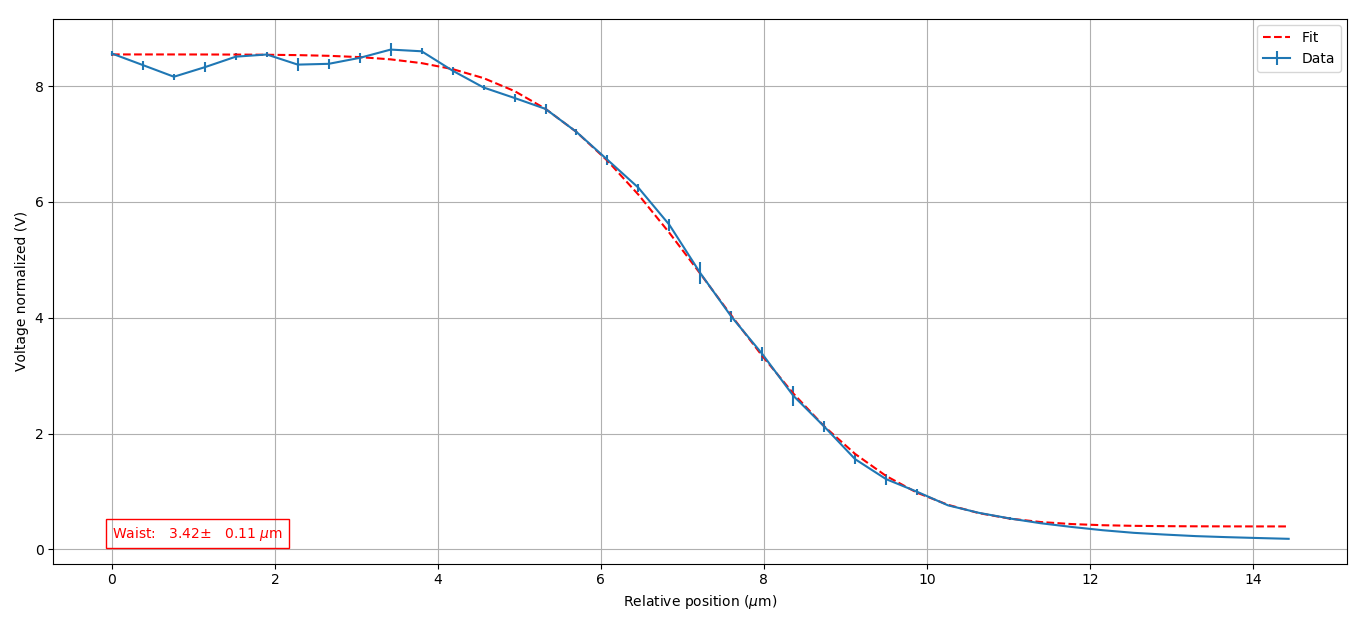
\includegraphics[width=\textwidth]{img/prova7}
\caption{Example of razor scan}
\end{figure}
\begin{figure}[H]
\centering
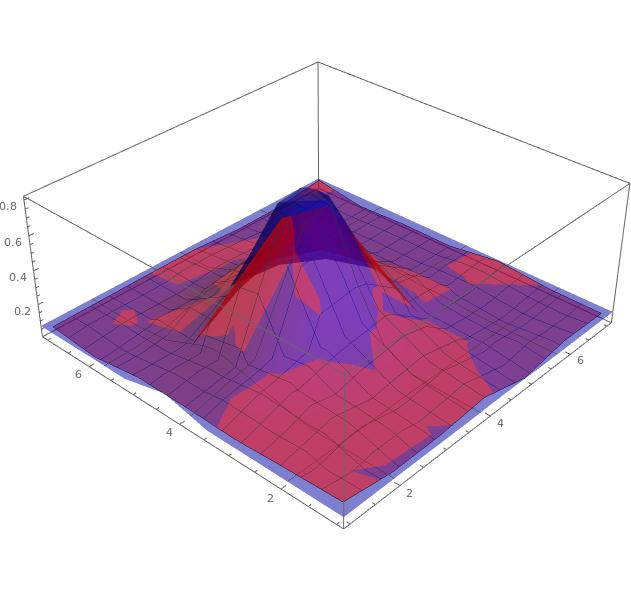
\includegraphics[width=\textwidth]{img/camera}
\caption{Example of camera picture}
\end{figure}
\subsection{Polarization characterization}
\subsection{Stability}
\section{Final installed system}
\subsection{Ramsey interferometry}
\begin{figure}[H]
\centering
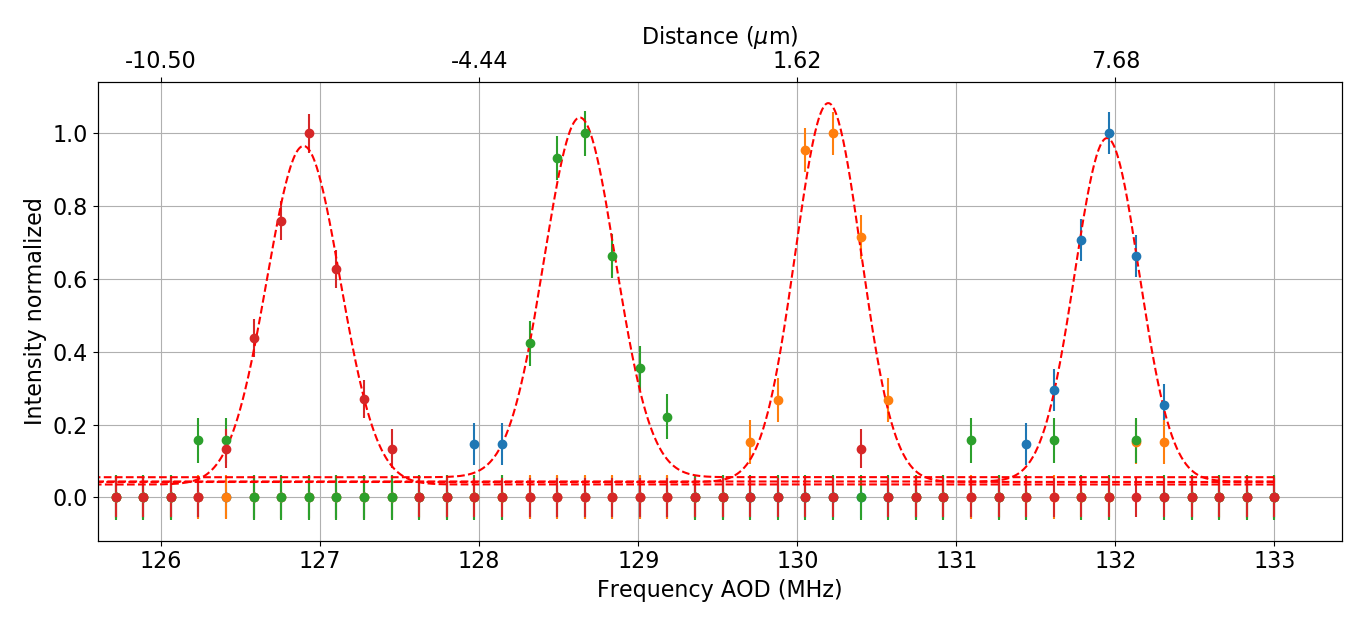
\includegraphics[width=\textwidth]{img/AODscan}
\caption{3 ions scanned}
\end{figure}
\begin{figure}[H]
\centering
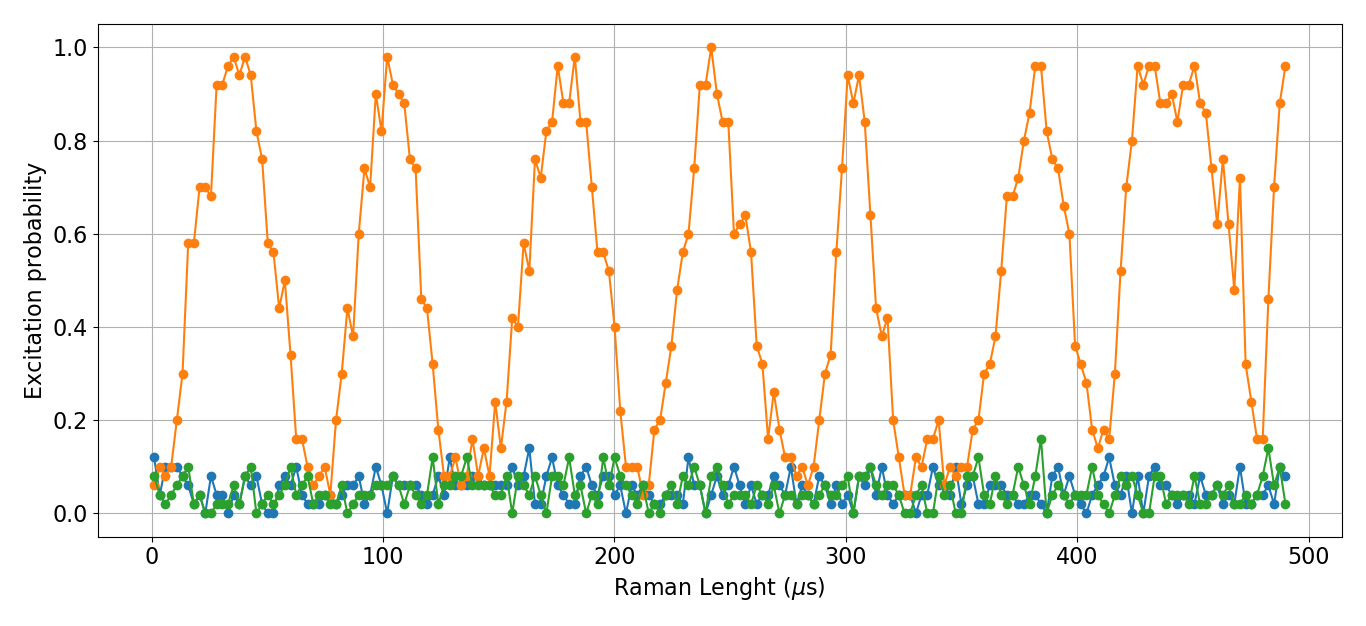
\includegraphics[width=\textwidth]{img/ac_stark}
\caption{393nm AC-Stark flops}
\end{figure}

\subsection{Photons production}
\begin{figure}[H]
\centering
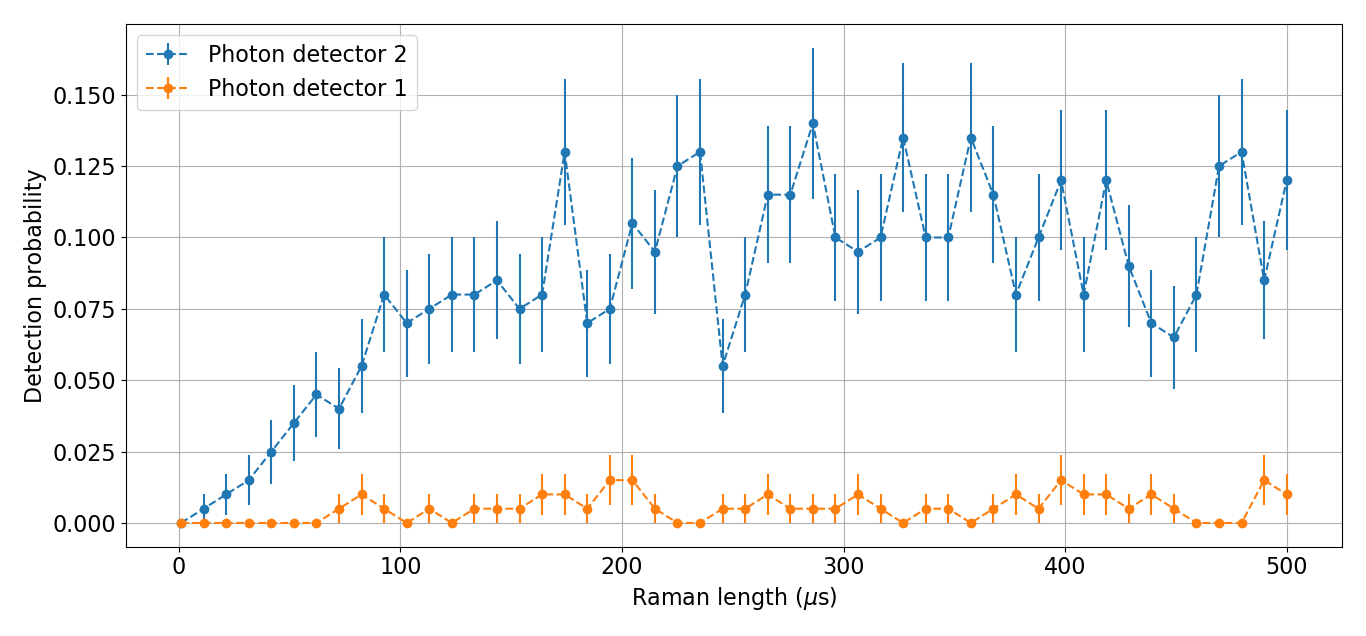
\includegraphics[width=\textwidth]{img/photonefficency_witherror}
\caption{Generated photon efficency}
\end{figure}

\begin{figure}[H]
\centering
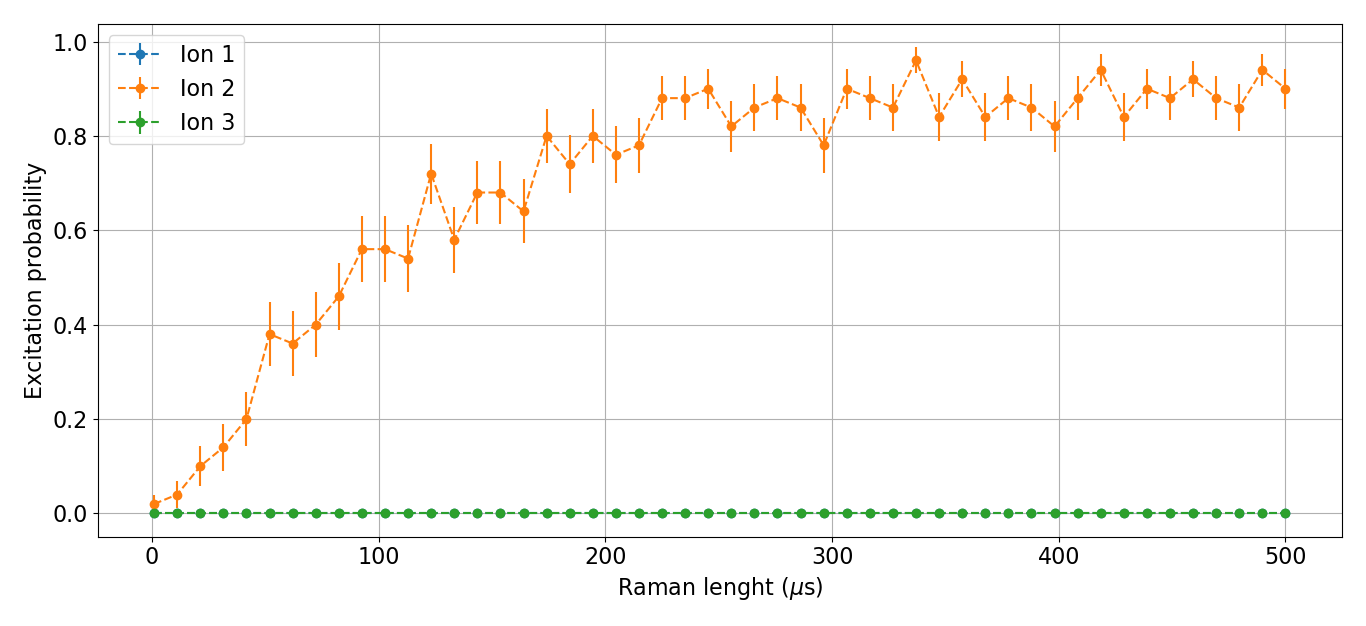
\includegraphics[width=\textwidth]{img/ramanlength_witherrors}
\caption{Excitation of ion while emitting photon}
\end{figure}

- g2 plot?
\section{Final properties summary}
